\documentclass[12pt,a4paper]{article}
\usepackage[utf8]{inputenc}
\usepackage{amsmath}
\usepackage{amsfonts}
\usepackage{amssymb}
\usepackage[brazil]{babel}
\usepackage{indentfirst}
\usepackage{url}

\usepackage{listings}
\usepackage{color}
\lstset{language=Python}
\definecolor{mygreen}{rgb}{0,0.6,0}
\definecolor{mygray}{rgb}{0.5,0.5,0.5}
\definecolor{mymauve}{rgb}{0.58,0,0.82}

\lstset{ %
  backgroundcolor=\color{white},   % choose the background color; you must add \usepackage{color} or \usepackage{xcolor}; should come as last argument
  basicstyle=\footnotesize,        % the size of the fonts that are used for the code
  breakatwhitespace=false,         % sets if automatic breaks should only happen at whitespace
  breaklines=true,                 % sets automatic line breaking
  captionpos=b,                    % sets the caption-position to bottom
  commentstyle=\color{mygreen},    % comment style
  deletekeywords={...},            % if you want to delete keywords from the given language
  escapeinside={\%*}{*)},          % if you want to add LaTeX within your code
  extendedchars=true,              % lets you use non-ASCII characters; for 8-bits encodings only, does not work with UTF-8
  frame=single,	                   % adds a frame around the code
  keepspaces=true,                 % keeps spaces in text, useful for keeping indentation of code (possibly needs columns=flexible)
  keywordstyle=\color{blue},       % keyword style
  language=Octave,                 % the language of the code
  morekeywords={*,...},            % if you want to add more keywords to the set
  numbers=left,                    % where to put the line-numbers; possible values are (none, left, right)
  numbersep=5pt,                   % how far the line-numbers are from the code
  numberstyle=\tiny\color{mygray}, % the style that is used for the line-numbers
  rulecolor=\color{black},         % if not set, the frame-color may be changed on line-breaks within not-black text (e.g. comments (green here))
  showspaces=false,                % show spaces everywhere adding particular underscores; it overrides 'showstringspaces'
  showstringspaces=false,          % underline spaces within strings only
  showtabs=false,                  % show tabs within strings adding particular underscores
  stepnumber=1,                    % the step between two line-numbers. If it's 1, each line will be numbered
  stringstyle=\color{mymauve},     % string literal style
  tabsize=2,	                   % sets default tabsize to 2 spaces
  title=\lstname                   % show the filename of files included with \lstinputlisting; also try caption instead of title
}
\RequirePackage{graphicx}
\title{Algoritmo Viola-Jones}
\author{Adallberto Lucena \and Andrey Silva \and Anny Karoliny \and Brener Gomes \and Davi Ildeu \and Eduardo de Oliveira \and Gleyson Israel \and Gusttavo Nunes \and Ianka Talita \and Ígor Justino}

 
\usepackage[left=3cm,right=3cm,top=2cm,bottom=2cm]{geometry}


\begin{document}
\begin{titlepage}


\begin{center}
\begin{figure}[htb]
		
		\label{figura:LogoIF}
	
		\centering
		
\includegraphics[width=6cm]{recursos/imagens/logo.png} 
\end{figure}


Instituto Federal Goiano - Campus Ceres\\
Bacharelado em Sistemas de Informação\\
Prof. Me. Ronneesley Moura Teles\\\vspace{0.5cm}
Adallberto Lucena Moura \\
Andrey Silva Ribeiro\\
Anny Karoliny Moraes Ribeiro \\
Brener Gomes de Jesus\\
Davi Ildeu de Faria\\
Eduardo de Oliveira Silva\\
Gleyson Israel Alves\\
Gusttavo Nunes Gomes\\
Ianka Talita Bastos de Assis\\
Ígor Justino Rodrigues\\



\vspace{5.0cm}

\textit{\textbf{\Large{Algoritmo Viola-Jones}}}\\\vspace{0.5cm}
\vspace{9.5cm}

Outubro\\
2017\\
\end{center}
\end{titlepage}



\tableofcontents

\newpage
\begin{center}
\textbf{\Large{Algoritmo Viola-Jones}}\\\vspace{0.5cm}
\end{center}

\section{Viola - Jones}
	O método \textit{Viola-Jones} proposto por \textit{Paul Viola} e \textit{Michael Jones} em 2001, é um algoritmo utilizado em diversas áreas da tecnologia, uma delas é a detecção de faces. Paul e Michael eram pesquisadores de Cambrigde onde optaram por explorar o lado radical da programação, sendo assim, publicaram um artigo intitulado: “\textit{Rapid Object Detection using a Boosted Cascade of Simple Features}” que demonstrou uma nova forma de detectar faces. O artigo bem como o conceito Viola-Jones faz uso de 3 abordagens diferenciadas, pautando pontos considerados de extrema importância, sendo eles: as características de \textit{Haar}, o algoritmo de aprendizado \textit{AdaBoost} e os classificadores em Cascata.

	As características de Haar proposta pelo matemático húngaro Alfred Haar em 1909, foi a primeira maneira considerada nova de representar uma “\textit{imagem integral}” (\textit{Integral Image}, em inglês), que permitiu os detectores utilizados por eles, computarem as imagens de forma rápida e eficaz. \textit{Haar} é uma característica intitulada como transformada onde varia da matemática discreta que faz uso em diversos processos de análises de sinais, em meios de compressão de dados e amplas outras aplicações no ramo de engenharia e ciência da computação.


	A segunda abordagem essencial foi o algoritmo de aprendizado baseado em \textit{AdaBoost}. O algoritmo AdaBoost é caracterizado por algoritmo de\textit{ Machine Learning} (aprendizado de máquina, em português) inventado por Yoav Freund e Robert Schapire, o algoritmo meta-heurístico é usado para aumentar significativamente a performance dos algoritmos de aprendizagem. \textit{AdaBoost} é derivado do nome \textit{Adaptive Boosting} (impulso adaptativo, significado em português) algoritmo colocado como ajustável a diversas circunstâncias e adaptável para classificações subsequentes. O algoritmo seleciona um número pequeno de características visuais críticas de um conjunto maior e com seus classificadores torna-se extremamente eficiente.

	Tendo em vista tais ferramentas úteis para elaboração do algoritmo, Paul e Michael implementaram os classificadores em Cascata. Os classificadores são responsáveis por selecionar criteriosamente um determinado objeto, levando em consideração a concomitância de suas principais características. As características necessárias para utilização são encontradas a partir de amplos algoritmos de aprendizado como \textit{Support Vector Machine}, redes neurais, entre outros. Os classificadores em cascata possuem como principal função combinar e incrementar métodos que tendenciam melhorar a perspectiva do objeto, ou seja, permitiam com que diversas regiões do fundo da foto fossem rapidamente destacadas disponibilizando maior processamento computacional.

	Por conseguinte, rejeitavam um largo número de regiões que demostravam ter o aspecto escolhido tornando-o então, cada vez mais prudente para que não ocorresse casos de falsos objetos nas análises dos mesmos. Os autores aprofundaram seus métodos de acordo com a construção do algoritmo, deste modo, realizaram comparações em relação a diferentes algoritmos similares da época, bem como, \textit{Rowley-Baluja-Kanade}, \textit{Schneiderman-Kanade} e\textit{ Roth-Yang-Ahuja} para que pudessem encontrar meios de solucionar a forma como funcionavam as equações e obter assim, resultados satisfatórios. 

	O algoritmo Viola-Jones é uma variação do \textit{AdaBoost}, algoritmo de aprendizado. Porém,por ser uma alternância, o algoritmo Viola-Jones é bastante utilizado. Devido sua implementação seguir uma abordagem diferente para construir um novo sistema de detecção, ele consegue alcançar aproximadamente 15 vezes mais rápido que os métodos anteriores. Viola-Jones é perfeitamente apto a detectar faces com maior precisão usando \textit{Haar} como uma das implementações, é notório a perspectiva que há em aplicar o algoritmo em diversas situações. O método Viola-Jones revolucionou o campo da computação tornando-se referência para os demais. 

\section{Funcionamento do algoritmo} 

\subsection{Integral Image}


\begin{figure}[h!]
\centering
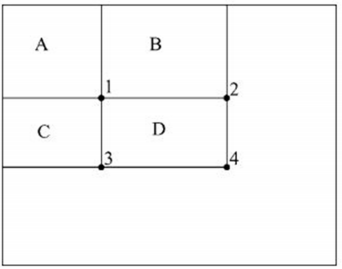
\includegraphics[width=5cm]{recursos/imagens/Integral.png}
\label{1}
\caption{Integral Image}
\end{figure} 

\subsection{Haar Feature}



\begin{figure}[h!]
\centering
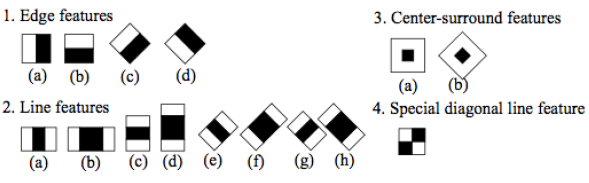
\includegraphics[width=5cm]{recursos/imagens/Haar.png}
\label{2}
\caption{Haar}
\end{figure} 

\begin{figure}[h!]
\centering
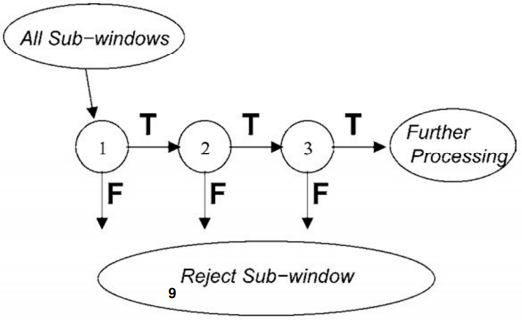
\includegraphics[width=5cm]{recursos/imagens/cascata.png}
\label{3}
\caption{Classificadores em Cascata}
\end{figure} 



\subsection{AdaBoost}







\section{Vantagem}
\begin{itemize}
	\item 15 vezes mais rápido que o algoritmo “\textit{Rowley-Baluja-Kanade}” no processamento da imagem.

	\item 600 vezes se comparado ao “\textit{Schneiderman-Kanade}”.
\end{itemize}

\section{Desvantagem}
\begin{itemize}
	\item A detecção de faces só é possível se o rosto estiver na posição frontal;
	\item A base de dados usada precisa de faces em diferentes condições, sendo elas: iluminação, brilho, escala, pose e variações de câmera;
	\item Nível de detecção na literatura - 80\% (FAUX,2012);
	\item É um algoritmo de detecção de face não de reconhecimento facial.
\end{itemize}

\section{Implementação Viola-Jones em Python}

\subsection{Por que a implementação em Python?}
	Existem inúmeras implementações do algoritmo disponíveis em plataformas confiáveis para utilização. Diversas linguagens foram desenvolvidas sendo elas as mais comuns em \textit{MatLab}, \textit{Java} e \textit{Python}. A implementação em MatLab não é de extrema significância ao se referir a detecção devido a ferramenta em si, não descartando sua utilização e benefícios para desenvolver procedimentos como o de detecção facial. Porém, é uma ferramenta paga e um projeto que demanda uma alta porcentagem de acertos e usabilidade, onde a interação de muitos indivíduos seriam colocados em pauta, viria deixar de ser uma solução para então tornar-se um problema se o usuário não obter a licença de uso, ou seja, dificultaria o processo e por delonga, devidamente descartado.  

	Java é uma linguagem abundante no \textit{GitHub}, entretanto a maioria estava incompleta ou não possui os códigos necessários para o treinamento da rede, o que faz-se importante para o sucesso do algoritmo e para que tenham uma base de dados ampla gerando uma maior eficiência na detecção de imagens. Os códigos aparentemente completos deixam a desejar a documentação estando assim, incoerentes ou inexistentes o que por sua vez, dificultou a utilização do mesmo, sendo mais vantajoso optar por uma ampliação do que gastar tempo em códigos alheios. 

	Deste modo, o método viável para implementação veio de \textit{Simon Hohberg} com o algoritmo em Python, que por conseguinte, encontra-se disponível no \textit{Github} pessoal do desenvolvedor:
\url{https://github.com/Simon-Hohberg/Viola-Jones}. \textit{Python} é considerada uma linguagem simples, mas nem por isso menos robusta. Nota-se que é amplamente utilizada em processos de \textit{Machine Learning} (aprendizado de máquina, em português) e a implementação selecionada está com o algoritmo completo e documentação do código estruturada desde a detecção até o treinamento, havendo então, a possibilidade de utilização. 



\subsection{IntegralImage.py}


 \lstinputlisting[language=Python]{recursos/codigo_python/Viola-Jones-master/violajones/IntegralImage.py}
 
 \subsection{HaarLikeFeature.py}

 \lstinputlisting[language=Python]{recursos/codigo_python/Viola-Jones-master/violajones/HaarLikeFeature.py}

\subsection{AdaBoost.py}
\lstinputlisting[language=Python]{recursos/codigo_python/Viola-Jones-master/violajones/AdaBoost.py}

\subsection{Utils.py}

\lstinputlisting[language=Python]{recursos/codigo_python/Viola-Jones-master/violajones/Utils.py}




%\lstinputlisting[language=Python, firstline=37, lastline=45]{source_filename.py}


\newpage
\section{Referências Bibliográfica}
\noindent VIOLA, Paul; JONES, Michael. \textbf{Rapid object detection using a boosted cascade of simple features.} Proceedings of the 2001 IEEE Computer Society Conference on Computer Vision and Pattern Recognition. CVPR 2001, v. 1, p. I-511-I-518, 2001. Disponível em: $<$\url{http://ieeexplore.ieee.org/document/990517/}$>$.\\\vspace{0.2cm}

\noindent VIOLA, Paul; JONES, Michael. \textbf{Robust Real-Time Face
Detection}  International Journal of Computer Vision
57(2), 137–154, 2004.\\\vspace{0.2cm}


\noindent CHAVES, Bruno Butilhão. \textbf{Estudo do algoritmo AdaBoost de aprendizagem de máquina aplicado a sensores e sistemas embarcados}. 2011. Dissertação (Mestrado em Engenharia de Controle e Automação Mecânica) - Escola Politécnica, Universidade de São Paulo, São Paulo, 2011. doi:10.11606/D.3.2011.tde-12062012-163740. Acesso em: 2017-10-11..\\\vspace{0.2cm}


\noindent IRGENS, Peter et al. \textbf{An efficient and cost effective FPGA based implementation of the Viola-Jones face detection algorithm.} HardwareX, v. 1, p. 68–75, 2017. Disponível em: $<$\url{http://linkinghub.elsevier.com/retrieve/pii/S2468067216300116}$>$.\\\vspace{0.2cm}

\noindent SANTOS, Ligneul. \textbf{Detecção de faces através do algoritmo de Viola-Jones}. Coppe/Ufrj, 2011.\\\vspace{0.2cm}

\noindent FAUX, Francis e LUTHON, Franck. \textbf{Theory of evidence for face detection and tracking}. International Journal of Approximate Reasoning, v. 53, n. 5, p. 728–746, 2012. Disponível em: $<$\url{http://dx.doi.org/10.1016/j.ijar.2012.02.002}$>$.\\\vspace{0.2cm}

\noindent BODHI, S. R. e NAVEEN, S. \textbf{Face detection, registration and feature localization experiments with RGB-D face database}. Procedia Computer Science, v. 46, n. Icict 2014, p. 1778–1785, 2015. Disponível em: $<$\url{http://dx.doi.org/10.1016/j.procs.2015.02.132}$>$.







\end{document}

%Modelo de código para inserir figura

%\begin{figure}[h]
%\centering
%
\includegraphics[width=15cm]{logo.png}
%\label{4}
%\caption{Fonte:http://...; Acesso em 07/10/2017}
%\end{figure}